\documentclass{article}
\usepackage[margin=1in]{geometry}
\usepackage[T1]{fontenc}
\usepackage{csquotes}
\usepackage{url}
\usepackage{graphicx}
\usepackage{caption}
\usepackage{xcolor,colortbl}
\usepackage{textcomp} 
\usepackage{listings}
\usepackage{enumitem}
\usepackage{float}
\usepackage{subfig}
\usepackage{hyperref}
\usepackage{indentfirst}
\renewcommand{\familydefault}{\sfdefault}

\newcommand{\mc}[2]{\multicolumn{#1}{c}{#2}}
\definecolor{Gray}{gray}{0.95}
\definecolor{LightCyan}{rgb}{0.88,1,1}

\newcolumntype{a}{>{\columncolor{Gray}}l}
\newcolumntype{b}{>{\columncolor{white}}c}

\graphicspath{{./img/}}


% Listings

\lstset{numbers=none,numberblanklines=false,columns=fullflexible,basicstyle=\ttfamily,linewidth=\columnwidth,breaklines=true}

\newcommand{\CodeSymbol}[1]{\bfseries\textcolor{violet}{#1}}   % Code associated to defining styles
\newcommand{\InitColor}[1]{\bfseries\textcolor{orange}{#1}}   % Code associated to defining styles
\newcommand{\RedColor}[1]{\bfseries\textcolor{red}{#1}}   % Code associated to defining styles
\newcommand{\PairColor}[1]{\bfseries\textcolor{blue}{#1}}   % Code associated to defining styles
\newcommand{\CustomFunction}[1]{\bfseries\textcolor{magenta}{#1}}   % Code associated to defining styles

\definecolor{codegray}{gray}{0.95}
\definecolor{commentgray}{gray}{0.35}

\makeatletter

\lstdefinelanguage{clingo}{%
  basicstyle=\footnotesize\ttfamily,%
  backgroundcolor=\color{codegray},%
  showstringspaces=false,%
  alsoletter=0123456789,%
  columns=fullflexible,%
  resetmargins=true,%
  breaklines=true,%
  keywords=[3]{&,&dom,&sum,&diff,&show},%
  morecomment=[l]{\#\ },%
  morecomment=[l]{\%\ },%
  morestring=[b]",%
  stringstyle={\itshape},%
  commentstyle={\color{commentgray}},%
  literate={init}{{\InitColor{init}}}1
           {not}{{\RedColor{not }}}1
           {pair}{{\PairColor{pair}}}1
           {onNode}{{\CustomFunction{onNode}}}1
           {occurs}{{\CustomFunction{occurs}}}1
           {action}{{\CustomFunction{action}}}1
           {move}{{\CodeSymbol{move}}}1
           {robot}{{\CodeSymbol{robot}}}1
           {robotMove}{{\CustomFunction{robotMove}}}1
           {onRobot}{{\CustomFunction{onRobot}}}1
           {deliver}{{\CustomFunction{deliver}}}1
           {onShelf}{{\CustomFunction{onShelf}}}1
           {order}{{\CustomFunction{order}}}1
           {goal}{{\CustomFunction{goal}}}1
           {pickingStation}{{\CustomFunction{pickingStation}}}1
           {nodeAt}{{\CodeSymbol{nodeAt}}}1
           {object}{{\CodeSymbol{object}}}1
           {value}{{\CodeSymbol{value}}}1
           {\#const}{{\CodeSymbol{\#const }}}1
           {\#show}{{\CodeSymbol{\#show }}}1
           {\#minimize}{{\CodeSymbol{\#minimize }}}1
           {\#base}{{\CodeSymbol{\#base }}}1
           {\#theory}{{\CodeSymbol{\#theory }}}1
           {\#count}{{\CodeSymbol{\#count }}}1
           {\#external}{{\CodeSymbol{\#external }}}1
           {\#program}{{\CodeSymbol{\#program }}}1
           {\#script}{{\CodeSymbol{\#script }}}1
           {\#end}{{\CodeSymbol{\#end }}}1
           {\#heuristic}{{\CodeSymbol{\#heuristic }}}1
           {\#edge}{{\CodeSymbol{\#edge }}}1
           {\#project}{{\CodeSymbol{\#project }}}1
           {\#show}{{\CodeSymbol{\#show }}}1
           {\#sum}{{\CodeSymbol{\#sum }}}1%
}

\newcommand\opstyle{\CodeSymbol} % <--- customise operator style here

% Hook into listings
\lst@AddToHook{OutputOther}{\ProcessOther@silmeth}

% helper macro
\newcommand\ProcessOther@silmeth
{%
  \ifnum\lst@mode=\lst@Pmode%     % If we're in `Processing' mode...
    \def\lst@thestyle{\opstyle}%  % ... redefine the style locally
  \fi%
}

\makeatother

\newcommand{\Sim}{{\raise.17ex\hbox{\ensuremath{\scriptstyle\sim}}}}

\begin{document}

\title{SER 334: Linux Kernel Modules}
\author{Claudio Rodriguez Rodriguez}
\maketitle

% task_struct - from <linux/sched.h> <-- defined here

% for_each_process - from <linux/sched/signal.h> <-- defined here (MACRO)

% list_for_each - from #include <linux/list.h> <-- defined here (MACRO)
% list_entry - from #include <linux/list.h>  <-- defined here (MACRO)
% list_head - from #include <linux/list.h>

% module_param - from #include <linux/moduleparam.h> <-- defined here (MACRO)
% MODULE_PARM_DESC - from #include <linux/moduleparam.h> <-- defined here (MACRO)

% printk - from <linux/kernel.h> 
% defined in #include <linux/printk.h>
% function

% print_header
% print_row
% init_rodriguez_rodriguez_lkm_module
% exit_rodriguez_rodriguez_lkm_module

Module 5 Programming Exercise is about Implementing a Loadable Kernel Module in 
Linux to display details about the processes executing in the kernel. 

\section{Kernel Version}

The Kernel Code used for reference was version \href{https://git.kernel.org/pub/scm/linux/kernel/git/stable/linux.git/snapshot/linux-5.13.19.tar.gz.}{5.13.19}, 
and the Linux Kernel used to run the Module on the Operating System is 5.13.0-27-generic.

\section{Main Source File}

The main source of the module is in the file \texttt{RodriguezRodriguezLKM.c}.
The output desired from the LKM is shown in Figure~\ref{fig:expectedOutput}. 
The Module must be able to take an optional parameter \texttt{inp\_pid} on insertion.\\

\begin{figure}[h!]
  \centering
  \captionsetup{justification=centering}
  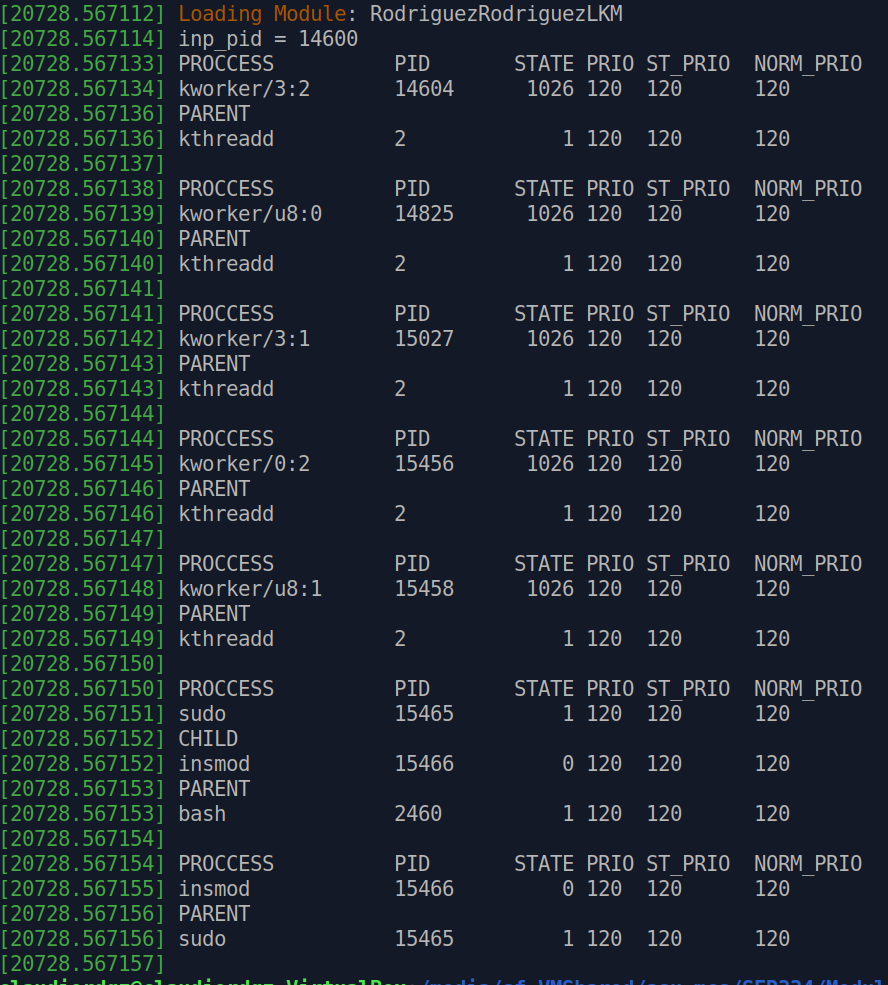
\includegraphics[width=0.5\textwidth]{screenshotOutput1.png}
  \caption{
    Expected output from LKM.
  }%
  \label{fig:expectedOutput}%
\end{figure}

The following functions were defined to achieve the functionality.\\

\fbox{\begin{minipage}{30em}
  \underline{\texttt{init\_rodriguez\_rodriguez\_lkm\_module}}\\
  Defined on line 67 in \texttt{RodriguezRodriguezLKM.c}.\\
  \textbf{Signature:}\\
  \texttt{int init\_rodriguez\_rodriguez\_lkm\_module(void);}.\\
  \textbf{Parameters:} None.\\
  \textbf{Description:} The entry-point of a Linux Kernel Module to be used with \texttt{sudo insmod *.ko} file.
\end{minipage}}
\\

\fbox{\begin{minipage}{30em}
  \underline{\texttt{exit\_rodriguez\_rodriguez\_lkm\_module}}\\
  Defined on line 94 in \texttt{RodriguezRodriguezLKM.c}.\\
  \textbf{Signature:} \texttt{void exit\_rodriguez\_rodriguez\_lkm\_module(void);}.\\
  \textbf{Parameters:} None.\\
  \textbf{Description:} The exit-point of a Linux Kernel Module to be used with \texttt{sudo rmmod *.ko} file.
\end{minipage}}
\\

\fbox{\begin{minipage}{30em}
  \underline{\texttt{print\_header}}\\
  Defined on line 98 in \texttt{RodriguezRodriguezLKM.c}.\\
  \textbf{Signature:} \texttt{void print\_header(void);}.\\
  \textbf{Parameters:} None.\\
  \textbf{Description:} A utility function to co-locate the \texttt{printk} format specifier close to the \texttt{print\_row} function to match the sizes of the columns between them.
\end{minipage}}
\\

\fbox{\begin{minipage}{30em}
  \underline{\texttt{print\_row}}.=\\
  Defined on line 102 in \texttt{RodriguezRodriguezLKM.c}.\\
  \textbf{Signature:}\\
  \texttt{void print\_row(struct task\_struct *task);}.\\
  \textbf{Parameters:} A pointer to the task\_struct data which allows us to reuse the print statement.\\
  \textbf{Description:} A utility function to reuse when printing the information related to the current process, children, or its parent without repeating too much information.
\end{minipage}}
\\

\section{task\_struct}

The \texttt{task\_struct} data structure is defined in the file \texttt{include/linux/sched.h}.\\

\begin{itemize}
  \item \texttt{PROCESS NAME}: Retrieved from the \texttt{comm} field of the \texttt{task\_struct} data structure. Per the code, its max length is 16 characters.
  \item \texttt{PID}: Retrieved from the \texttt{pid} field of the \texttt{task\_struct} data structure. We use \texttt{cat \/proc\/sys\/kernel\/pid\_max} to determine the length of the column.
  \item \texttt{STATE}: Retrieved from the \texttt{state} field of the \texttt{task\_struct} data structure.
  \item \texttt{PRIORITY}: Retrieved from the \texttt{prio} field of the \texttt{task\_struct} data structure.
  \item \texttt{STATIC-PRIORITY}: Retrieved from the \texttt{static\_prio} field of the \texttt{task\_struct} data structure.
  \item \texttt{NORMAL-PRIORITY}: Retrieved from the \texttt{normal\_prio} field of the \texttt{task\_struct} data structure.
  \item \texttt{CHILDREN}: Retrieved from the \texttt{children} field of the \texttt{task\_struct} data structure and utility macros to navigate lists.
  \item \texttt{PARENT}: Retrieved from the \texttt{parent} field of the \texttt{task\_struct} data structure.
\end{itemize}

\section{Kernel Functions/Macros/Structs used}


\fbox{\begin{minipage}{30em}
  \underline{\texttt{task\_struct}}\\
  Struct defined on line 657 from <linux/sched.h>.\\
  \textbf{Signature:} \texttt{struct task\_struct}.\\
  \textbf{Parameters:} None.\\
  \textbf{Description:} The task\_struct is the primary representation of a Process in the Kernel code. The program uses the struct to retrieve the properties of the processes.
\end{minipage}}

\fbox{\begin{minipage}{30em}
  \underline{\texttt{for\_each\_process}}\\
  Macro defined on line 607 from <linux/sched/signal.h>.\\
  \textbf{Signature:} \texttt{\#define for\_each\_process(p)}.\\
  \textbf{Parameters:} The macro receives an argument $p$ which is an uninitialized pointer to a \texttt{task\_struct}.\\
  \textbf{Description:} The macro uses the uninitialized pointer and it translates to a for loop that starts \texttt{\&init\_task}.
  The definition of \texttt{struct task\_struct init\_task} is on the file \texttt{init\\init\_task.c} on line 64 and it seems 
  to be the primordial task in the Kernel. The loop will navigate using the macro \texttt{next\_task} which also receives the pointer to the task.
\end{minipage}}

\fbox{\begin{minipage}{30em}
  \underline{\texttt{list\_for\_each}}\\
  Macro defined on line 570 from <linux/list.h>.\\
  \textbf{Signature:} \texttt{\#define list\_for\_each(p, head)}.\\
  \textbf{Parameters:} p is a uninitialized pointer to a \texttt{struct list\_head} and head is in this case the head of the list.\\
  \textbf{Description:} The \texttt{task\_struct} contains a children property of type \texttt{list\_head}. 
  This property used as the head parameter of this macro allows navigating the children's processes of a process.
\end{minipage}}

\fbox{\begin{minipage}{30em}
  \underline{\texttt{list\_entry}}\\
  Macro defined on line 510 from <linux/list.h>.\\
  \textbf{Signature:} \texttt{\#define list\_entry(ptr, type, member)}.\\
  \textbf{Parameters:}
  \begin{itemize}[noitemsep,topsep=0pt]
    \item ptr is a pointer to a \texttt{struct list\_head} that we used on \texttt{list\_for\_each}.
    \item type is the type of the struct, in our case \texttt{struct task\_struct}.
    \item member is the name of the struct's member, we already fetched the children of our task, so in this case we are interested in fetching the children sibling.
  \end{itemize}
  \textbf{Description:} A helper macro to retrieve the struct from this entry, the second parameter defined the type of struct to retrieve.
\end{minipage}}

\fbox{\begin{minipage}{30em}
  \underline{\texttt{list\_head}}\\
  Struct defined on line 178 from <linux/types.h>.\\
  \textbf{Signature:} \texttt{struct list\_head}.\\
  \textbf{Parameters:} None.\\
  \textbf{Description:} A utility struct to navigate a list, it contains pointers to the next and previous items in the list.
\end{minipage}}

\fbox{\begin{minipage}{30em}
  \underline{\texttt{module\_param}}\\
  Macro defined on line 126 from <linux/moduleparam.h>.\\
  \textbf{Signature:} \texttt{\#define module\_param(name, type, perm)}.\\
  \textbf{Parameters:} 
  \begin{itemize}[noitemsep,topsep=0pt]
    \item name is the name of existing variable we will use, in this case a static variable. 
    \item type is the type of the variable.
    \item perm is the permission of the parameter.
  \end{itemize}
  \textbf{Description:} This helper macro is very useful to define the parameters we pass to our module when doing module insertion (insmod).
\end{minipage}}

\fbox{\begin{minipage}{30em}
  \underline{\texttt{MODULE\_PARM\_DESC}}\\
  Macro defined on line 33 from <linux/moduleparam.h>.\\
  \textbf{Signature:} \texttt{\#define MODULE\_PARM\_DESC(name, desc)}.\\
  \textbf{Parameters:} 
  \begin{itemize}[noitemsep,topsep=0pt]
    \item name name of the param matching \texttt{module\_param}.
    \item desc is the description of the parameter.
  \end{itemize}
  \textbf{Description:} Macro to add documentation to \texttt{module\_param}, and useful to read using the Linux Command \texttt{modinfo}.
  An example of the documentation is seen on Figure~\ref{fig:modinfo}.
\end{minipage}}

\begin{figure}[h!]
  \centering
  \captionsetup{justification=centering}
  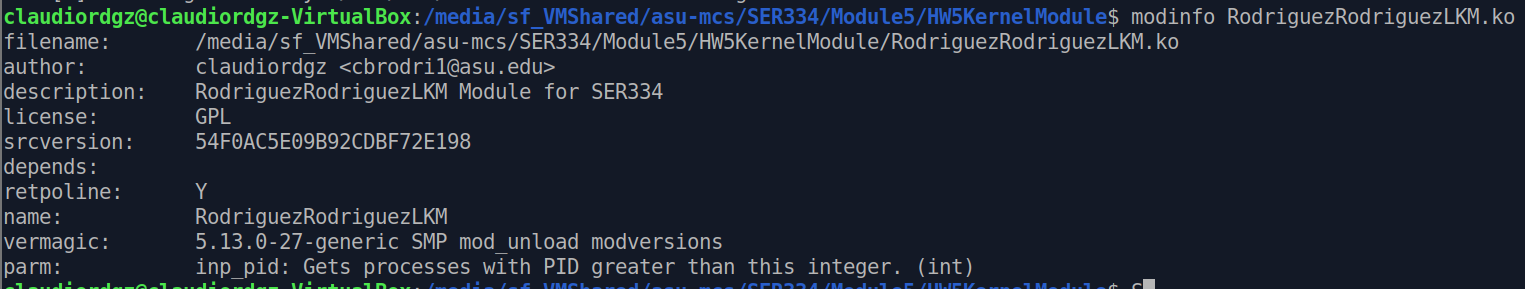
\includegraphics[width=\textwidth]{screenshotModInfo1.png}
  \caption{
    Modinfo output showing Module Param Description for inp\_pid.
  }%
  \label{fig:modinfo}%
\end{figure}

\fbox{\begin{minipage}{30em}
  \underline{\texttt{printk}}\\
  Function declared on line 176 of <linux/printk.h> and defined on line 2210 from kernel/printk/printk.c.\\
  \textbf{Signature:} \texttt{int printk(const char *fmt, ...);}.\\
  \textbf{Parameters:}
  \begin{itemize}[noitemsep,topsep=0pt]
    \item fmt is the format of the message.
    \item ... is the list of arguments.
  \end{itemize}
  \textbf{Description:} This function is similar to the printf function, but instead of printing to STD\_OUT, it prints to the kernel log. 
  It has the addition that you can add a prefix to the message to define the LOG\_LEVEL of the message.
\end{minipage}}

\end{document}
